\section{Auswertung}
\label{sec:Auswertung}
\subsection{Die $γ$-Absorption}
Der hier verwendete $\gamma$-Strahler ist $^{137}$Cs.
Bei der Nullmessung über $800\si{\second}$ ergab sich ein Wert von
\begin{align*}
Z_u=935\pm31
\intertext{gemessen. Dies entspricht einer Impulsrate von:}
N_u=(1,04\pm0,03)\si{\per\second}
\end{align*}
Der Fehler dieser und den folgenden Messungen entspricht $\sqrt{Z}$.
In den Tabelle sind die Messwerte für $\gamma$-Strahlung bei den Absorptionsmaterialien Kupfer \ref{tab:yCu}
und Blei \ref{tab:yPb} aufgelistet.
\begin{table}
  \centering
  \caption{Messwerte mit einer Kupferplatte.}
  \label{tab:yCu}
  \begin{tabular}{c c c c}
Zeit $s$ in $\si{\second}$& Impulse $Z$  & Dicke $D$ in \si{\milli\meter} & Impulsrate $N-N_u$ in $\si{\per\second}$\\
       \midrule
       40 & 6081\pm78 & 0,48\pm0,2 &151,0\pm1,9 \\
       40 & 5948\pm77 & 1,92\pm0,2 &147.7\pm1,9 \\
       40 & 4364\pm66 & 6,92\pm0,2 &108,1\pm1,7 \\
       40 & 5291\pm73 & 2,88\pm0,2 &131,2\pm1,8 \\
       40 & 3692\pm61 & 10\pm0,2   & 91,3\pm1,5 \\
       40 & 2370\pm49 & 20\pm0,2   & 58,2\pm1,2 \\
       40 & 1904\pm44 & 25\pm0,2   & 46,6\pm1,1 \\
       40 & 1411\pm38 & 30\pm0,2   & 34,2\pm0,9 \\
       40 & 1058\pm33 & 35\pm0,2   & 25,4\pm0,8 \\
       40 & 850\pm29  & 40\pm0,2   & 20,2\pm0,7 \\
       40 & 770\pm28  & 45\pm0,2   & 18,2\pm0,7 \\
       40 & 546\pm23  & 50\pm0,2   & 12,6\pm0,6 \\
       40 & 321\pm18  & 60\pm0,2   & 7,0\pm0,4 \\
      \bottomrule
    \end{tabular}
\end{table}
\begin{table}
  \centering
  \caption{Messwerte mit einer Bleiplatte.}
  \label{tab:yPb}
  \begin{tabular}{c c c c}
Zeit $s$ in $\si{\second}$& Impulse $Z$  & Dicke $D$ in \si{\milli\meter} & Impulsrate $N-N_u$ in $\si{\per\second}$ \\
       \midrule
       40  & 5583\pm75 & 1,4\pm0,2  & 138,5\pm1,9\\
       40  & 4965\pm70 & 2,8\pm0,2  & 123,1\pm1,8\\
       40  & 4456\pm67 & 4,2\pm0,2  & 110,4\pm1,7\\
       40  & 2059\pm45 & 10\pm0,2   & 50,4\pm1,1\\
       40  & 1509\pm39 & 14,2\pm0,2 & 36,7\pm1,0\\
       40  & 643\pm25  & 20\pm0,2   & 15,0\pm0,6\\
       40  & 451\pm21  & 24,2\pm0,2 & 10,2\pm0,5\\
       40  & 255\pm16  & 30\pm0,2   & 5,3\pm0,4 \\
       60  & 290\pm17  & 34,2\pm0,2 & 3,8\pm0,3\\
       100 & 318\pm18  & 40\pm0,2   & 2,1\pm0,2\\
       200 & 455\pm21  & 50\pm0,2   & 1,2\pm0,2\\
       300 & 351\pm19  & 60\pm0,2   & 0,1\pm0,1\\
      \bottomrule
    \end{tabular}
\end{table}
Aus diesen Tabellen werden nun
die Impulsrate $N-N_u$ in Abbhängigkeit von der Plattendicke $D$
aufgetragen. Die Abbildung \ref{fig:cu} enthält die
Messwerte für die Kupferplatten und Abbildung \ref{fig:pb}
die für die Bleiplatten.

\begin{figure}
  \centering
  \includegraphics[width=0.7\textwidth]{a)cu.pdf}
  \caption{Impulsrate $N$ in Abhängigkeit der Dicke $D$ der Kupferplatten.}
  \label{fig:cu}
\end{figure}

\begin{figure}
  \centering
  \includegraphics[width=0.7\textwidth]{a)pb.pdf}
  \caption{Impulsrate $N$ in Abhängigkeit der Dicke $D$ der Bleiplatten.}
  \label{fig:pb}
\end{figure}

Durch diese Messwerte wird nun versucht eine e-funktion in der Form
\begin{align*}
  N=A\cdot e^{C\cdot D}
\end{align*}
zu fitten.
Die Koeffizienten $A$ und $C$ entsprechen $N_0$ der Ausgangs-Impulsrate und $\mu$ der Absorptionskoeffizient aus dem Absorptionsgesetz \eqref{eqn:abs}.
Somit ergibt sich für die folgenden Werte aus der Messung für Kupfer:
\begin{align*}
N_{0_{Cu}}=(155,6\pm1,7)\si{\per\second},\\
\mu_{Cu}=(50,4\pm1,2)\si{\per\meter}\\
\intertext{und für Blei}
N_{0_{Pb}}=(166,8\pm3,2)\si{\per\second},\\
\mu_{Pb}=(112,0\pm4,0)\si{\per\meter}.
\end{align*}

\subsection{Theoretische Berechnung des Compton-Absorptionskoeffizienten}
Die verwendete $^{137}$Cs-Strahlung besitzt eine relative Energie $\epsilon$ von
\begin{align*}
  \epsilon=1,295.
\end{align*}
Über diese und dem klassischen Elektronenradius $r_e$, welcher $2,82\cdot10^{-15}\si{\meter}$
beträgt, lässt sich nun mit der Formel \eqref{eqn:sigma}
der Wirkungsquerschnitt $\sigma_\mathrm{Com}$ für die Comption-Streuung
berechnen.
\begin{align*}
\sigma_\mathrm{Com}=25,7\cdot10^{30}\si{\meter\tothe{2}}
\end{align*}

Nun kann durch den Zusammenhang aus der Formel \eqref{eqn:mucom} der
Apsorptionskoeffizienten $\mu_\mathrm{com}$ berechnet werden:
\begin{align}
\mu_\mathrm{com}=\frac{zN_A}{V_\mathrm{Mol}}\sigma_\mathrm{com}.\label{eqn:mucom}
\end{align}
%??Wobei $N_l$ die Loschmidtsche Zahl ist.
%\begin{align*}
%N_L=2,6867811\cdot10^{25}\si{\per\meter\tothe{3}}\text{\cite{constants}}
%\end{align*}
Dafür werden noch die
Kernladungszahl $z$ und das Molvolumen $V_\mathrm{Mol}$ der
verwendeten Materialien benötigt.
Die Werte für Kupfer sind:
\begin{align*}
z_{Cu}&=29\\
V_{M_{Cu}}&=7,11 \cdot 10^{-6}\si{\meter\tothe{3}\per\mol} \text{\cite{chemiecu}}.
\intertext{Somit ergibt sich ein Absorptionskoeffizient $\mu_\mathrm{Com}$ für Kupfer:}
\mu_\mathrm{Com_{cu}}&={63,02\si{\per\meter}}.
\intertext{Die Werte für Blei sind:}
z_{Pb}&=82\\
V_{M_{Pb}}&=18,26 \cdot 10^{-6}\si{\meter\tothe{3}\per\mol} \text{ \cite{chemiepb}}.
\intertext{Daraus ergibt sich ein Absorptionskoeffizient $\mu_\mathrm{Com}$ für Blei von:}
  \mu_\mathrm{Com_{pb}}&={69,38\si{\per\meter}}.
\end{align*}

\subsection{ $β$-Absorption}

Die Tablelle \ref{tab:b} enthält die
Messwerte für einer $\beta$-Quelle hier $^{99}Tc$
und dem Absorptionsmaterial Aluminium.
Wobei die Nullmessung über $900\si{\second}$ den folgenden Wert lieferte:
\begin{align*}
Z_u&=292\pm17.
\intertext{Dies entspricht einer Impulsrate von:}
N_u&=(0,324\pm0,019)\si{\per\second}.
\end{align*}
Diese wird wieder, wie bei der $\gamma$-Strahlung, von der gemessen Impulsrate $N$ abgezogen.
\begin{table}
  \centering
  \caption{Messwerte bei dem Absorbtionsmaterial Aluminium.}
  \label{tab:b}
  \begin{tabular}{c c c c}
Zeit $s$ in $\si{\second}$& Impulse $Z$  & Dicke $D$ in \si{\micro\meter} & Impulsrate $N-N_u$ in $\si{\per\second}$\\
       \midrule
       40  & 1386\pm37  & 102\pm1   &34,33\pm0,93   \\
       40  &  665\pm26  & 126\pm1   &16,30\pm0,64 \\
       60  &  431\pm21  & 153\pm0.5 &6,86\pm0,35 \\
       100 &  462\pm21  & 160\pm1   &4,30\pm0,22 \\
       250 &  287\pm17  & 200\pm1   &0,82\pm0,68 \\
       400 &  269\pm16  & 253\pm1   &0,35\pm0,07 \\
       650 &  241\pm16  & 302\pm1   &0,07\pm0,05 \\
       800 &  419\pm20  & 338\pm5   &0,20\pm0,03 \\
       700 &  333\pm18  & 400\pm1   &0,15\pm0,03 \\
       800 &  497\pm22  & 444\pm2   &0,30\pm0,03 \\
       800 &  441\pm21  & 482\pm1   &0,23\pm0,03 \\
      \bottomrule
    \end{tabular}
\end{table}
\FloatBarrier
Diesmal wird die Impulsrate $N$ in Abhängigkeit
von der Massenbelgung $R$ aufgetragen wie in der Abbildung \ref{fig:b} zu sehen.
die Massenbelgung ergibt sich aus der Zusammenhang:
\begin{align*}
  R=\rho D
\end{align*}
Wobei die Dichte $\rho$ von Aluminium
\begin{align*}
  \rho_\mathrm{Al}=2,7\si{\gram\per\centi\meter\tothe{3}}\text{\cite{chemieal}}
\end{align*}
beträgt.
Die y-Achse wird diesmal logarithmisch aufgetragen, dadurch
lassen sich die Messwerte in zwei lineare Bereiche einteilen
wie in Abblidung \ref{fig:b} verdeutlich wird.
\begin{figure}
  \centering
  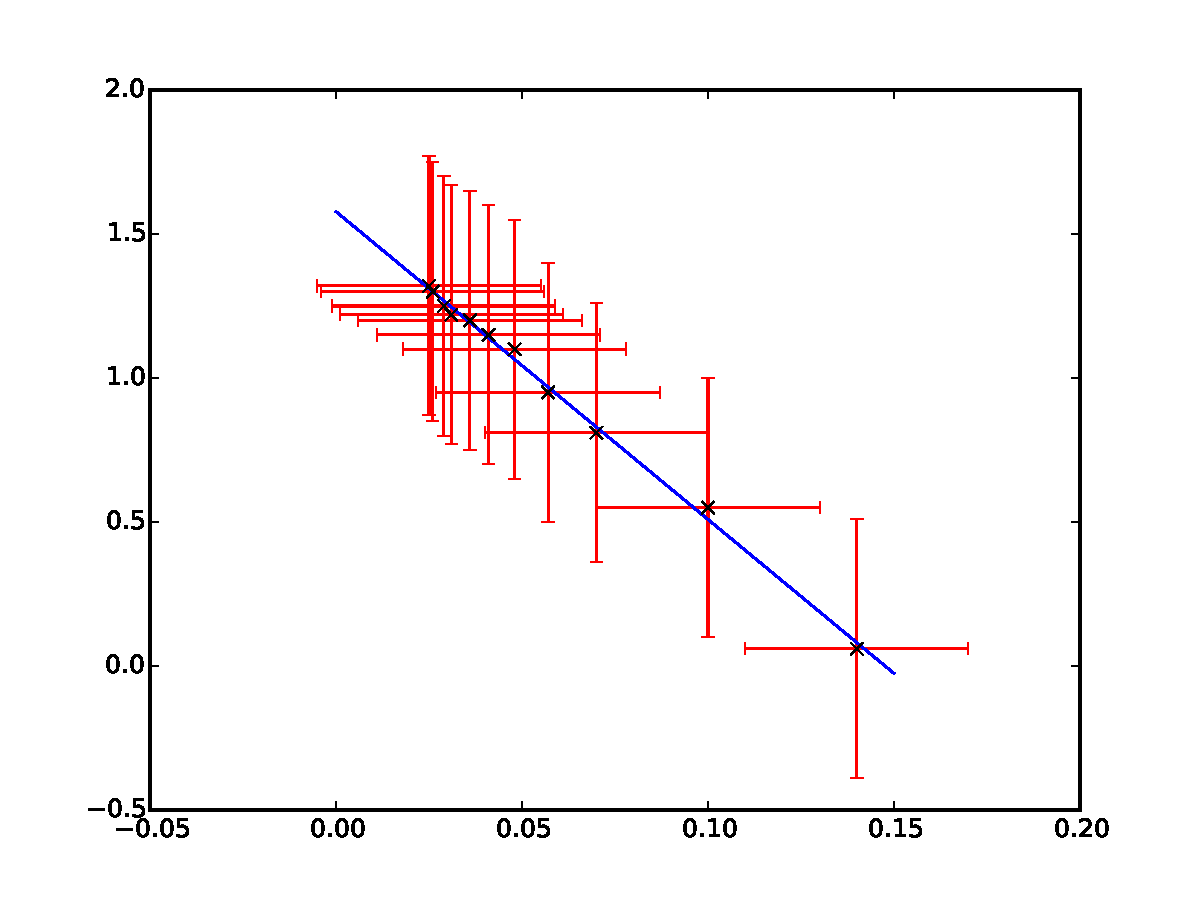
\includegraphics[width=0.7\textwidth]{b).pdf}
  \caption{Logarithmierte Impulsrate $N$ in Abhängigkeit der Dicke $D$ der Aluminiumplatten.}
  \label{fig:b}
\end{figure}
\FloatBarrier
Um nun die maximale Reichweite $R_{max}$ der $\beta$-Teilchen bestimmen zu können, wird eine
lineare Regression in beiden
Bereichen durchgeführt und es ergeben sich zwei Geraden in der Form von:
\begin{align*}
  y&=A_\mathrm{i}x+B_\mathrm{i}
\intertext{Mit den Parametern:}
A_1&=-14,1\pm0,8,\\
B_1&=7,56\pm0,33,\\
A_2&=0,7\pm1,5,\\
B_2&=-2,4\pm1,5.
\end{align*}

Mit Hilfe dieser Parameter lässt sich nun über die Formel \eqref{eqn:rmax}
$R_{max}$ bestimmen.
\begin{align}
R_{max}&=\frac{B_2-B_1}{A_1-A_2}\label{eqn:rmax}
\intertext{Somit ergibt sich ein $R_{max}$ von:}
R_{max}&=(0,67\pm0,13)\si{\gram\per\centi\meter\tothe{2}}.
\end{align}
Über $R_{max}$ kann nun die beim $\beta$-Zerfall freiwerdende Gesamtenergie
$E_\mathrm{max}$ durch einsetzen in die Formel \eqref{eqn:emax} bestimmt werden.
Es ergibt sich ein $E_\mathrm{max}$ von:
\begin{align*}
  E_{max}=(1,49\pm0,25)\si{\mega\electronvolt}.
\end{align*}
